\chapter{Introduzione}
\label{Introduzione}
\thispagestyle{empty}

%\begin{quotation}
%	{\footnotesize
%		\noindent\emph{``Terence: Mi fai un gelato anche a me? Lo vorrei di pistacchio. \\
%			Bud: Non ce l'ho il pistacchio. C'ho la vaniglia, cioccolato, fragola, limone e caff\`e. \\
%			Terence: Ah bene. Allora fammi un cono di vaniglia e di pistacchio. \\
%			Bud: No, non ce l'ho il pistacchio. C'ho la vaniglia, cioccolato, fragola, limone e caff\`e. \\
%			Terence: Ah, va bene. Allora vediamo un po', fammelo al cioccolato, tutto coperto di pistacchio. \\
%			Bud: Ehi, macch\'e sei sordo? Ti ho detto che il pistacchio non ce l'ho! \\
%			Terence: Ok ok, non c'\`e bisogno che t'arrabbi, no? Insomma, di che ce l'hai? \\
%			Bud: Ce l'ho di vaniglia, cioccolato, fragola, limone e caff\`e! \\
%			Terence: Ah, ho capito. Allora fammene uno misto: mettici la fragola, il cioccolato, la vaniglia, il limone e il caff\`e. Charlie, mi raccomando il pistacchio, eh.''}
%		\begin{flushright}
%			Pari e dispari
%		\end{flushright}
%	}
%\end{quotation}
%\vspace{0.5cm}
Una branca dell'industria tecnologica che sta prendendo sempre pi\`u piede \`e quella dei \textit{sistemi di monitoraggio video}.
L'abbattimento dei costi delle camere e una sempre maggiore integrazione di tecnologie hardware con sensori e infrastrutture di rete hanno permesso una rapida crescita di questo settore.\\
Inoltre, il grande successo di Internet degli ultimi anni ha permesso l'utilizzo dei sistemi di monitoraggio video per applicazioni che prima non erano neanche pensabili.
Oggigiorno \`e possibile avere un sistema di videosorveglianza domestico spendendo poche centinaia di euro, controllabile con il proprio \textit{smartphone} attraverso Internet, oppure \`e possibile vedere le condizioni meteorologiche o del traffico nella propria citt\`a attraverso le immagini riprese da una \textit{webcam}.
Un servizio di questo genere \`e fornito da molte piattaforme web di previsioni del tempo.
Ad esempio, il sito \textit{ilMeteo.it} \cite{ilmeteo} permette di vedere in tempo reale il contenuto video di webcam presenti nelle principali citt\`a o in localit\`a di interesse turistico.\\
Uno dei maggiori problemi quando si ha a che fare con sistemi di monitoraggio video consiste nell'identificazione di particolari eventi in grado di compromettere la corretta ripresa della scena da parte del sensore.\\
%Eventi di questo tipo sono, ad esempio, lo spostamento della camera, oppure una scorretta messa a fuoco della scena.\\
Questo tipo di eventi viene classificato generalmente sotto il nome di \textit{tampering}, dall'inglese \textit{manomissione}.
Il termine deriva dal fatto che, di solito, questi eventi sono legati ad azioni intenzionali atte a impedire che la camera riprenda correttamente la scena.
Pu\`o succedere, ad esempio, che un ladro copra l'obiettivo della camera con qualche oggetto, in modo da poter agire indisturbato, oppure che la sposti in modo che riprenda qualcos'altro.
In questa tesi definiamo con il termine tampering un qualsiasi evento, intenzionale o meno, che possa compromettere la corretta acquisizione della scena inquadrata dalla camera.
Ad esempio una sfocatura pu\`o essere causata da dell'acqua piovana che si deposita a ridosso della lente, oppure pu\`o succedere che una folata di forte vento sposti la camera, cambiando quindi l'inquadratura della scena.\\
Questa definizione permette di analizzare il problema anche per quelle applicazioni di monitoraggio video che non sono direttamente legate alla videosorveglianza, ad esempio per lo scenario delle webcam introdotto sopra, in cui l'evento non \`e necessariamente dovuto a un intervento umano intenzionale.\\
Le tecniche algoritmiche che vengono utilizzate per identificare gli eventi di tampering prendono il nome di algoritmi di \textit{tampering detection}.\\
La letteratura scientifica ha prodotto molte soluzioni a riguardo, ma la maggior parte sono legate ad applicazioni di videosorveglianza.
Questo particolare tipo di applicazioni ha bisogno di camere che acquisiscano a framerate \textit{continuo}, solitamente tra i 30 frame per secondo (fps) e i 2 fps.
\`E infatti impensabile che una camera di videosorveglianza possa acquisire, ad esempio, un frame ogni minuto.\\
Lo scopo della tesi \`e lo sviluppo di un algoritmo di tampering detection per camere intelligenti (\textit{smart camera}) e a basso consumo.
In particolare abbiamo considerato scenari in cui la camera operi a \textit{basso framerate}, ad esempio acquisendo un'immagine ogni minuto.\\
Questa assunzione copre in realt\`a molti casi d'uso gi\`a esistenti, che non sono legati alla videosorveglianza.
\begin{figure}[t]
	\centering
	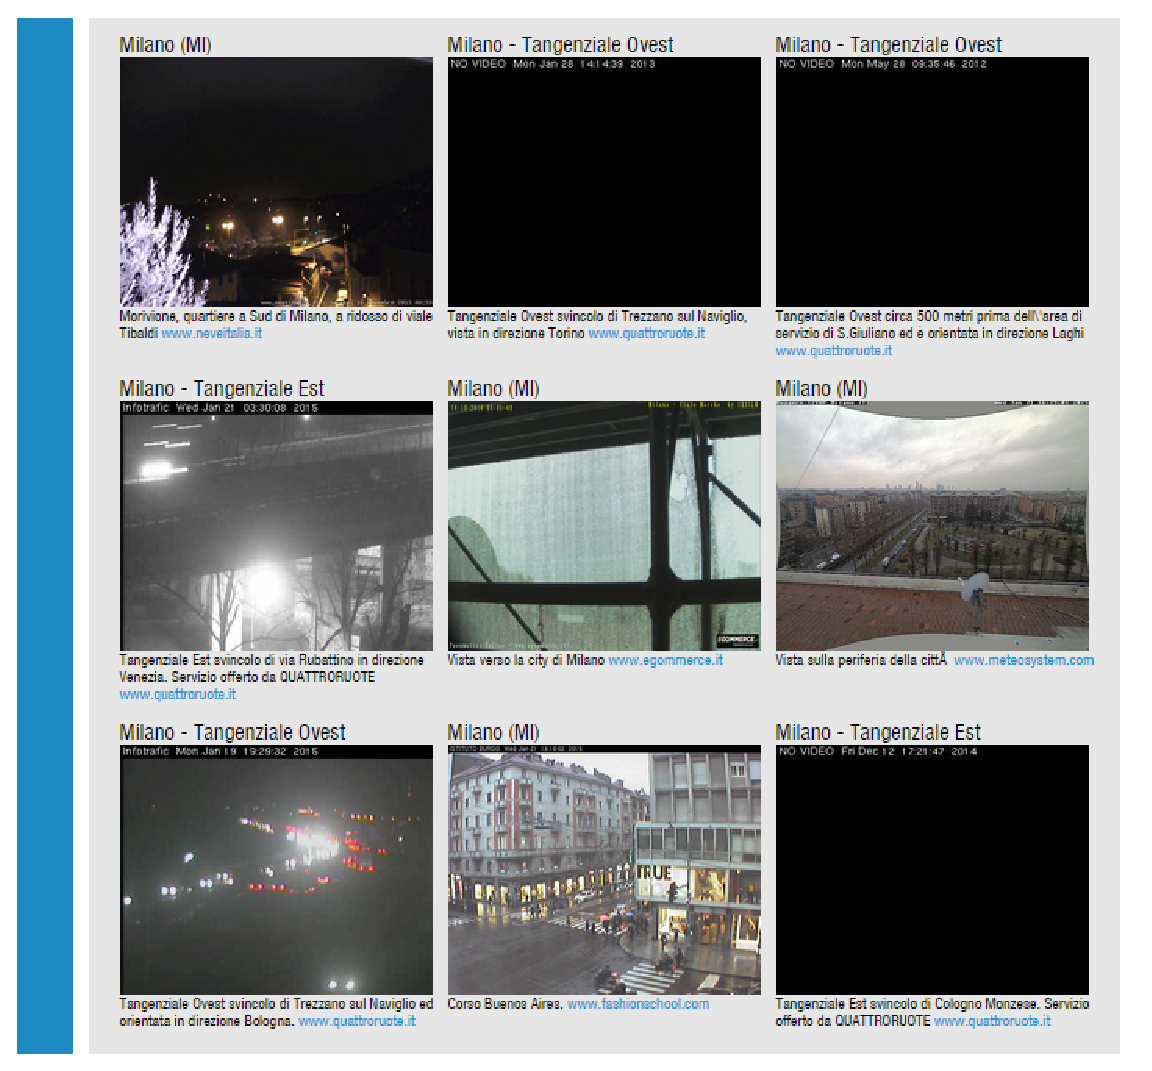
\includegraphics[width=12cm]{pictures/ilMeteo}
	\caption[Webcam per il monitoraggio meteorologico]{In questa figura vediamo un esempio di applicazione per sistemi di monitoraggio video. Molti siti di previsioni del tempo consentono l'accesso alle immagini registrate da webcam utilizzate per il monitoraggio meteorologico. Come possiamo vedere, la webcam al centro dell'immagine non \`e in condizioni di riprendere correttamente la scena, in quanto c'\`e un'impalcatura che ne impedisce la visione. Inoltre, possiamo vedere come alcune webcam non riprendano alcuna scena.}
	\label{fig:ilMeteo}
\end{figure}
Un esempio \`e quello delle webcam per il monitoraggio meteorologico che abbiamo illustrato precedentemente.
Nella Figura \ref{fig:ilMeteo} possiamo vedere come una parte delle webcam accessibili da un sito di previsioni del tempo in realt\`a non forniscano molte informazioni riguardanti il monitoraggio meteorologico:
alcune webcam sono spente, e quindi non inviano frame alla piattaforma, e una camera, quella centrale, non pu\`o riprendere la scena perch\'e le \`e stata posta un'impalcatura davanti.
Avere delle tecniche in grado di identificare in maniera automatica questo tipo di eventi potrebbe evitare l'invio di immagini compromesse e inviare un segnale di allarme al gestore della camera, che provvederebbe alla risoluzione del problema, ad esempio cambiando la locazione della camera.
In questo modo si aumenterebbe l'affidabilit\`a del sistema e si diminuirebbe il traffico di dati sulla rete, in quanto si eviterebbe di inviare frame compromessi.\\

Le tecniche principalmente utilizzate nella letteratura scientifica hanno come base il confronto di ciascun frame con quelli successivi, utilizzando \textit{modelli di background}.
Queste, per essere efficaci, hanno bisogno che i frame vengano acquisiti a framerate continuo, in quanto viene fatta l'ipotesi che tra i vari frame della scena il contenuto vari poco.
Abbiamo notato, invece, che operando a basso framerate le differenze tra frame consecutivi sono molto elevati, a causa di cambiamenti di luminosit\`a, di ombre e di zone dinamiche della scena.\\
Il nostro lavoro di tesi \`e una prosecuzione del lavoro svolto da \cite{alippi2010detecting}, dove vengono identificati eventi di sfocatura utilizzando \textit{tecniche sequenziali} su un indicatore \textit{scalare} estratto da ciascun frame.\\
Il nostro lavoro si \`e concentrato sugli eventi di \textit{sfocatura} e di \textit{spostamento della camera}.
Per individuare questi eventi analizziamo il comportamento di indicatori scalari estratti dalle singole immagini.
Abbiamo notato come questi eventi determinino un cambiamento molto brusco nel normale andamento di questi indicatori.


\noindent La tesi \`e strutturata nel seguente modo.\\
Nel Capitolo \ref{StatoArte} illustriamo le principali tecniche di identificazione di tampering presenti nella letteratura scientifica, introducendo anche alcuni principi di visione artificiale e di elaborazione di immagini necessari alla comprensione del resto della trattazione.\\
Nel Capitolo \ref{FormulazioneProblema} diamo una definizione formale degli eventi di tampering e del problema che si pone l'algoritmo di tampering detection.\\
Nel Capitolo \ref{SoluzioneProposta} illustriamo la soluzione al problema dell'identificazione degli eventi di tampering proposta da noi, entrando nel merito sui dettagli realizzativi.\\
Nel Capitolo \ref{ProveSperimentali} mostriamo le prove realizzate per validare la soluzione proposta, descrivendo anche la realizzazione dei dataset e i risultati ottenuti.\\
Nel Capitolo \ref{Conclusioni}, infine, tiriamo le conclusioni, descrivendo le prospettive future di ricerca.
	
